\documentclass[11pt]{article}
\usepackage[margin=1in]{geometry}
\usepackage{graphicx}
\usepackage{microtype}
\usepackage{verbatim}
\usepackage{amsmath}
\usepackage{nicefrac}
\usepackage[colorlinks=false, hidelinks]{hyperref}
\usepackage{caption}
\usepackage{subcaption}
\usepackage{listings}
\usepackage{harmony}
\usepackage{wasysym}

\begin{document}

\title{The Last Music Trainer\\Embedded System Design, Lab 4}
\date{October 8, 2015}
\author{Ben Lorenzetti}
\maketitle

\tableofcontents

\clearpage

\section{Objectives and Problem Descriptions}
\subsection{Beginner Music Trainer}
\label{problem-specs}

The objective of this lab is to develop microcontroller-based, beginner music trainer 
with the following features:
\begin{enumerate}

\item Be capable of playing simple songs using PBasic's 
\mbox{\texttt{FREQOUT Pin, Duraction, Freq1 \{, Freq2\}}} command.
This including the ability to
\begin{enumerate}
\item[a.] play any piano tone in the $4^{\textrm{th}}$--$7^{\textrm{th}}$ octave
\{C, C\#, D, D\#, E, F, F\#, G, G\#, A, A\#, B\};

\item[b.] change the base tempo's whole note duration;

\item[c.] play each note for \{1, $\nicefrac{1}{2}$, $\nicefrac{1}{4}$, $\nicefrac{1}{8}$,
$\nicefrac{1}{16}$, $\nicefrac{1}{32}$\} of the base tempo;

\item[d.] play each note for $1\frac{1}{2}*\{1$, $\nicefrac{1}{2}$, $\nicefrac{1}{4}$, $\nicefrac{1}{8}$, 
$\nicefrac{1}{16}$, $\nicefrac{1}{32}$\} (dotten notes) of the base tempo; and
\end{enumerate}

\item allow user to select from a menu of 5 Ring Tone Text Transfer Language
(RTTTL) songs,
using a pushbutton switch--each push causes an advance to the next song.

\item allow user to increase the base tempo by a factor of 1--4 using a potentiometer rotary knob.

\item display the current note being played on a 7-segment display,
using the decimal point to indicate sharp notes.
Furthermore, display the note's octave with individual LEDs.

\item play each song in an infinite loop if user does not advance to the next song.
\end{enumerate}

\section{Procedure}

\subsection{Circuit Design}

\begin{figure}
\centering
	\begin{subfigure}[b]{.2\textwidth}
		\centering
		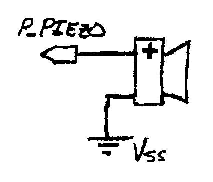
\includegraphics[width=\textwidth]{piezo-circuit.pdf}
		\caption[]%
		{{\small Piezo Circuit}}
	\end{subfigure}
	\quad
	\begin{subfigure}[b]{0.45\textwidth}
		\centering
		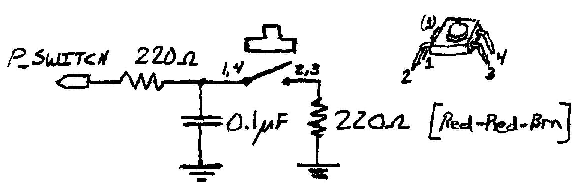
\includegraphics[width=\textwidth]{pushbutton-circuit.pdf}
		\caption[]%
		{{Pushbutton Switch Circuit}}
	\end{subfigure}
	\vskip\baselineskip
	\begin{subfigure}[b]{0.45\textwidth}
		\centering
		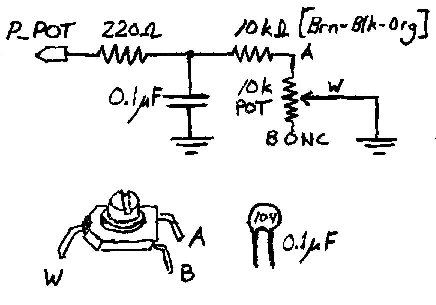
\includegraphics[width=\textwidth]{potentiometer-circuit.pdf}
		\caption[]%
		{{Potentiometer RC Circiut}}
	\end{subfigure}
	\quad
	\begin{subfigure}[b]{0.45\textwidth}
		\centering
		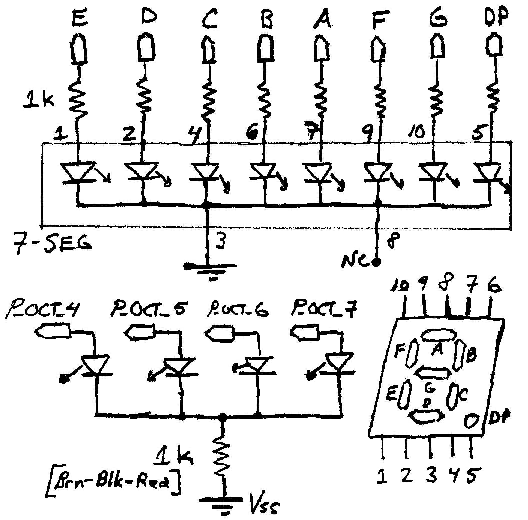
\includegraphics[width=\textwidth]{LED-display-circuit.pdf}
		\caption[]%
		{{LED Display Circuit}}
	\end{subfigure}	
	\caption{Hardware for The Last Music Trainer}
	\label{circuit-diagrams}
\end{figure}

Objectives 1-4 from the problem specifications (\hyperref[problem-specs]{section \ref{problem-specs}})
each require some hardware for their functionality.
Playing simple songs requires a piezo element, user song selection requires a pushbutton,
adjusting the base tempo requires a rotary potentiometer knob, and
displaying the current note requires a 7-segment display.

The circuit diagram for these 4 hardware sections are shown in
\hyperref[circuit-diagrams]{figure \ref{circuit-diagrams}}. 

For the pushbutton circuit, a capacitor is added in parallel to the switch;
if the capacitor is charged immediately after reading the pin, this capacitive
switch will have memory in case the switch is contacted while the controller
is busy.

For the rotary potentiometer, the RC time constant was found in a prior lab to be
\begin{equation}
\tau = \left[ \frac{0.06365R_{pot}}{\Omega}+636.5 \right] *[2\mu s]
\end{equation}

The time constant is given in units of 2 $\mu$s because that is the measurement
unit of the PBasic Stamp controller. The potentiometer resistance has a domain
of 0 $\Omega$-10 k$\Omega$, resulting in an expected range of 636.5-1273.
The and the range needs to be mapped linearly to a
speed factor of 1--4 and, from experience in the last lab, there should be built in
tolerance in case the time measurement is outside the expected range.
This can be done with the mapping
\begin{equation}
y=\frac{1}{256}\left( \frac{\tau}{[2\mu s]}-443 \right) +1
\end{equation}

\subsection{Data Design}

\begin{table}
\centering
\caption{10-Bit Note Encoding Truth Table}
\resizebox{\textwidth}{!}{
\begin{tabular}{c | c c | c | c | c | c c | c | c}
\hline
Length				&$*$	&Bit Code	&Dec.	&Whole Note Divisor	&Letter		&\#	&Bit Code	&Dec.	&$7^{\textrm{th}}$ Octave Freq	\\
\hline\hline
{\Huge \fullnote \par}		&0	&000		&0	&$(1<<0)$		&A$\natural$	&0	&000		&0	&3520.0	\\
\hline
{\Huge \fullnote \Pu \par}	&1	&000		&8	&			&A$\sharp$	&1	&000		&8	&3729.3	\\
\hline
{\Huge \halfnote \par}		&0	&001		&1	&$(1<<1)$		&B$\natural$	&0	&001		&1	&3951.1	\\
\hline
{\Huge \halfnote \Pu \par}	&1	&001		&9	&			&C$\natural$	&0	&010		&2	&2093.0	\\
\hline
{\Huge \quarternote \par}	&0	&010		&2	&$(1<<2)$		&C$\sharp$	&1	&010		&10	&2217.5	\\
\hline
{\Huge \quarternote \Pu \par}	&1	&010		&10	&			&D$\natural$	&0	&011		&3	&2349.3	\\
\hline
{\Huge \Acht \par}		&0	&011		&3	&$(1<<3)$		&D$\sharp$	&1	&011		&11	&2489.0	\\
\hline
{\Huge \Acht \Pu \par}		&1	&011		&11	&			&E$\natural$	&0	&100		&4	&2637.0	\\
\hline
{\Huge \Sech \par}		&0	&100		&4	&$(1<<4)$		&F$\natural$	&0	&101		&5	&2793.8	\\
\hline
{\Huge \Sech \Pu \par}		&1	&100		&12	&			&F$\sharp$	&1	&101		&13	&2960.0	\\
\hline
{\Huge \Zwdr \par}		&0	&101		&5	&$(1<<5)$		&G$\natural$	&0	&110		&6	&3136.0	\\
\hline
{\Huge \Zwdr \Pu \par}		&1	&101		&13	&			&G$\sharp$	&1	&110		&14	&3322.4	\\
\hline
				&	&		&	&			&P	&x	&111		&7,15	&-\\
\hline\hline
&&&&&	Octave				&	&Bit Code	&Dec.	&$7^{\textrm{th}}$ Freq. Divisor	\\
\hline\hline
&&&&&	$4^{\textrm{th}}$		&	&00		&0	&$1<<(3-0)$	\\
&&&&&	$5^{\textrm{th}}$		&	&01		&1	&$1<<(3-1)$	\\
&&&&&	$6^{\textrm{th}}$		&	&10		&2	&$1<<(3-2)$	\\
&&&&&	$7^{\textrm{th}}$		&	&11		&3	&$1<<(3-3)$	\\
\hline
\end{tabular}}
\label{data-lookup-table}
\end{table}

For this project, many songs will have to be stored in the Stamp's nonvolatile
EEPROM memory. The smaller the format of the song data, the better, because
more-and longer-songs will be able to be played.
Based on the full set of possible notes from the specification in
\hyperref[problem-specs]{section \ref{problem-specs}} and on the RTTTL data format,
the full information for a single note can be encoded in 10 bits.

A single note is encoded according to the following scheme:
\begin{verbatim}
Bits[9:8] = Note Octave
Bit [7]   = Sharp Flag
Bits[6:4] = Note Letter
Bit [3]   = Dotted Flag
Bits[2:0] = Note Type (whole, half, etc.)
\end{verbatim}
For example, listed most-significant bit first, the note \texttt{00|1|001|0|010 = 146}
would be octave=00, sharp=1, letter=1, dotted=0, and note\_type=010.
The mapping of the bit codes to physical, musical quantities are shown in
\hyperref[data-lookup-table]{table \ref{data-lookup-table}}.

For a full song, the data is encoded according to the following byte scheme:
\begin{verbatim}
[Song X Base Tempo Byte] [Song Length Byte] [Data Byte 0] [Data Byte 1] ...
... [Data Byte N] [Song X+1 Base Tempo Byte]...
\end{verbatim}
There are two bytes for the song meta data, a base tempo of 0-255 beats per minute and song length of 0-255 notes.
The number of data bytes is $N=\textrm{number of notes}*\frac{\textrm{10bits/note}}{\textrm{8 bits/byte}}$.
If the size of the data does not fall on a byte boundary, N is rounded up to the nearest integer and the
extra bits are padded with zeros. The next song starts at byte N+1.

The bit and byte packing orders are both least significant first.
For example, take bytes 0-4 of Let it Be by the Beatles.
\begin{verbatim}
|  B0=100  |  B1=26   |  B2=68   |  B3=206   | B4=40     |
| 00100110 | 01011000 | 00100010 | 01 110011 | 0001 0100 |
|Base Tempo|-#of Notes|----Note 0----|---Note 1----|-Low 4 Bits of Note 2 |
| 00100110 | 01011000 | 00100010   01|110011   0001|0100                  |
\end{verbatim}
For human decoding, Note 0 is rewritten with its most-significant bit first:
\begin{verbatim}
Note 0 = 1001000100; octave=10, sharp=0, letter=100, dotted=0, note_type=100
\end{verbatim}

\subsection{Data Generation from RTTTL Files}

It would be very monotonous to encode RTTTL songs to my 10-bit format by hand,
so I wrote a C script for automating the process. This program is included in
\hyperref[generate-rtttl-songs-section]{section \ref{generate-rtttl-songs-section}}.

\subsection{Implementation Flowchart}

\begin{figure}
\centering
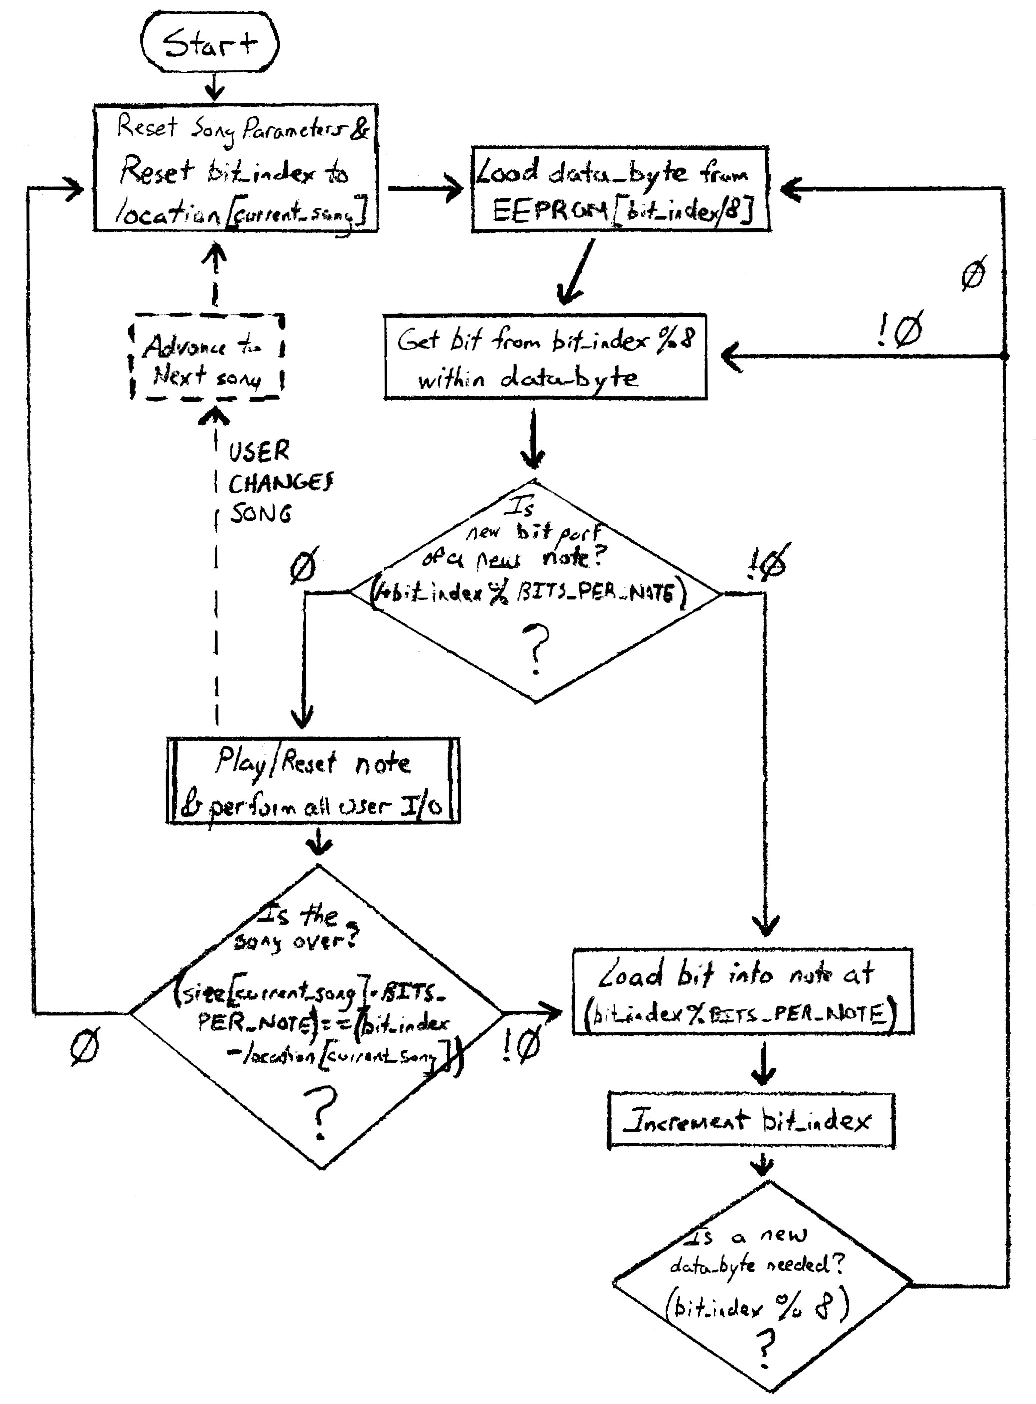
\includegraphics[width=0.8\textwidth]{music-trainer-flowchart.pdf}
\caption{Music Trainer Implementation Flowchart}
\label{music-trainer-flowchart}
\end{figure}

Unfortunately the minimum size for a note (10 bits) does not fall evenly
on a byte boundary. Therefore, there is a tradeoff between data compactness
and program complexity. I chose to prioritize data compactness, and the result
is a programming implementation with most of its complexity involved
in unpacking data.

The implementation flowchart is shown in
\hyperref[music-trainer-flowchart]{figure \ref{music-trainer-flowchart}}.
Most of the states and logic are dedicated to unpacking data in a bitwise
manner. The only states/transitions not involved in the bitwise unpacking
of data are shown as dotted lines in the flowchart.

\section{Expected Results}

\subsection{Laboratory Demonstration}

I expected my microcontroller and circuit to behave as described by the problem specifications in
\hyperref[problem-specs]{section \ref{problem-specs}}.
For the lab demonstration, the TA should be able to recognize at least 5 songs,
switch between songs with the pushbutton, change the song speed, and
see notes displayed on the 7-segment display and octave LEDs.

\section{Experiment and Design Revisions}

\subsection{Changes During Debugging}

During debugging, I spend some time fixing problems associated with the bit packing scheme.
There were three other bugs I fixed:

First, I was implementing pause notes as notes of zero frequency (\texttt{FREQOUT pin, duration, 0}),
but this resulting is a clicking noise that was unpleasent. I fixed this by wrapping the
\texttt{FREQOUT} statement with \text{IF (freq=0)} logic. 

Second, the songs were being played too fast. I fixed this by moving the speed factor
from the potentionmenter (1-4) from the denominator of the duration variable to the
numerator.

Third, an A note was being played at the beginning of every song. I fixed this by adding
an initialization value for \texttt{note} in the \text{Reset\_Song\_Parameters} state.

\section{Observations}

\subsection{Sound Intensity and Memory Mapping}

The last music trainer worked as expected after some initial debugging.
I did notice two interesting things. 
First, the piezo speaker seemed to play some notes louder than others.
Second, I looked at the memory map for my program and it seems my bit
packing scheme worked well--there was plenty of additional room for
more songs.

A photo of my music trainer and its memory map are shown in
\hyperref[the-music-trainer]{figure \ref{the-music-trainer}} and
\hyperref[memory-map]{figure \ref{memory-map}}.

\begin{figure}
\centering
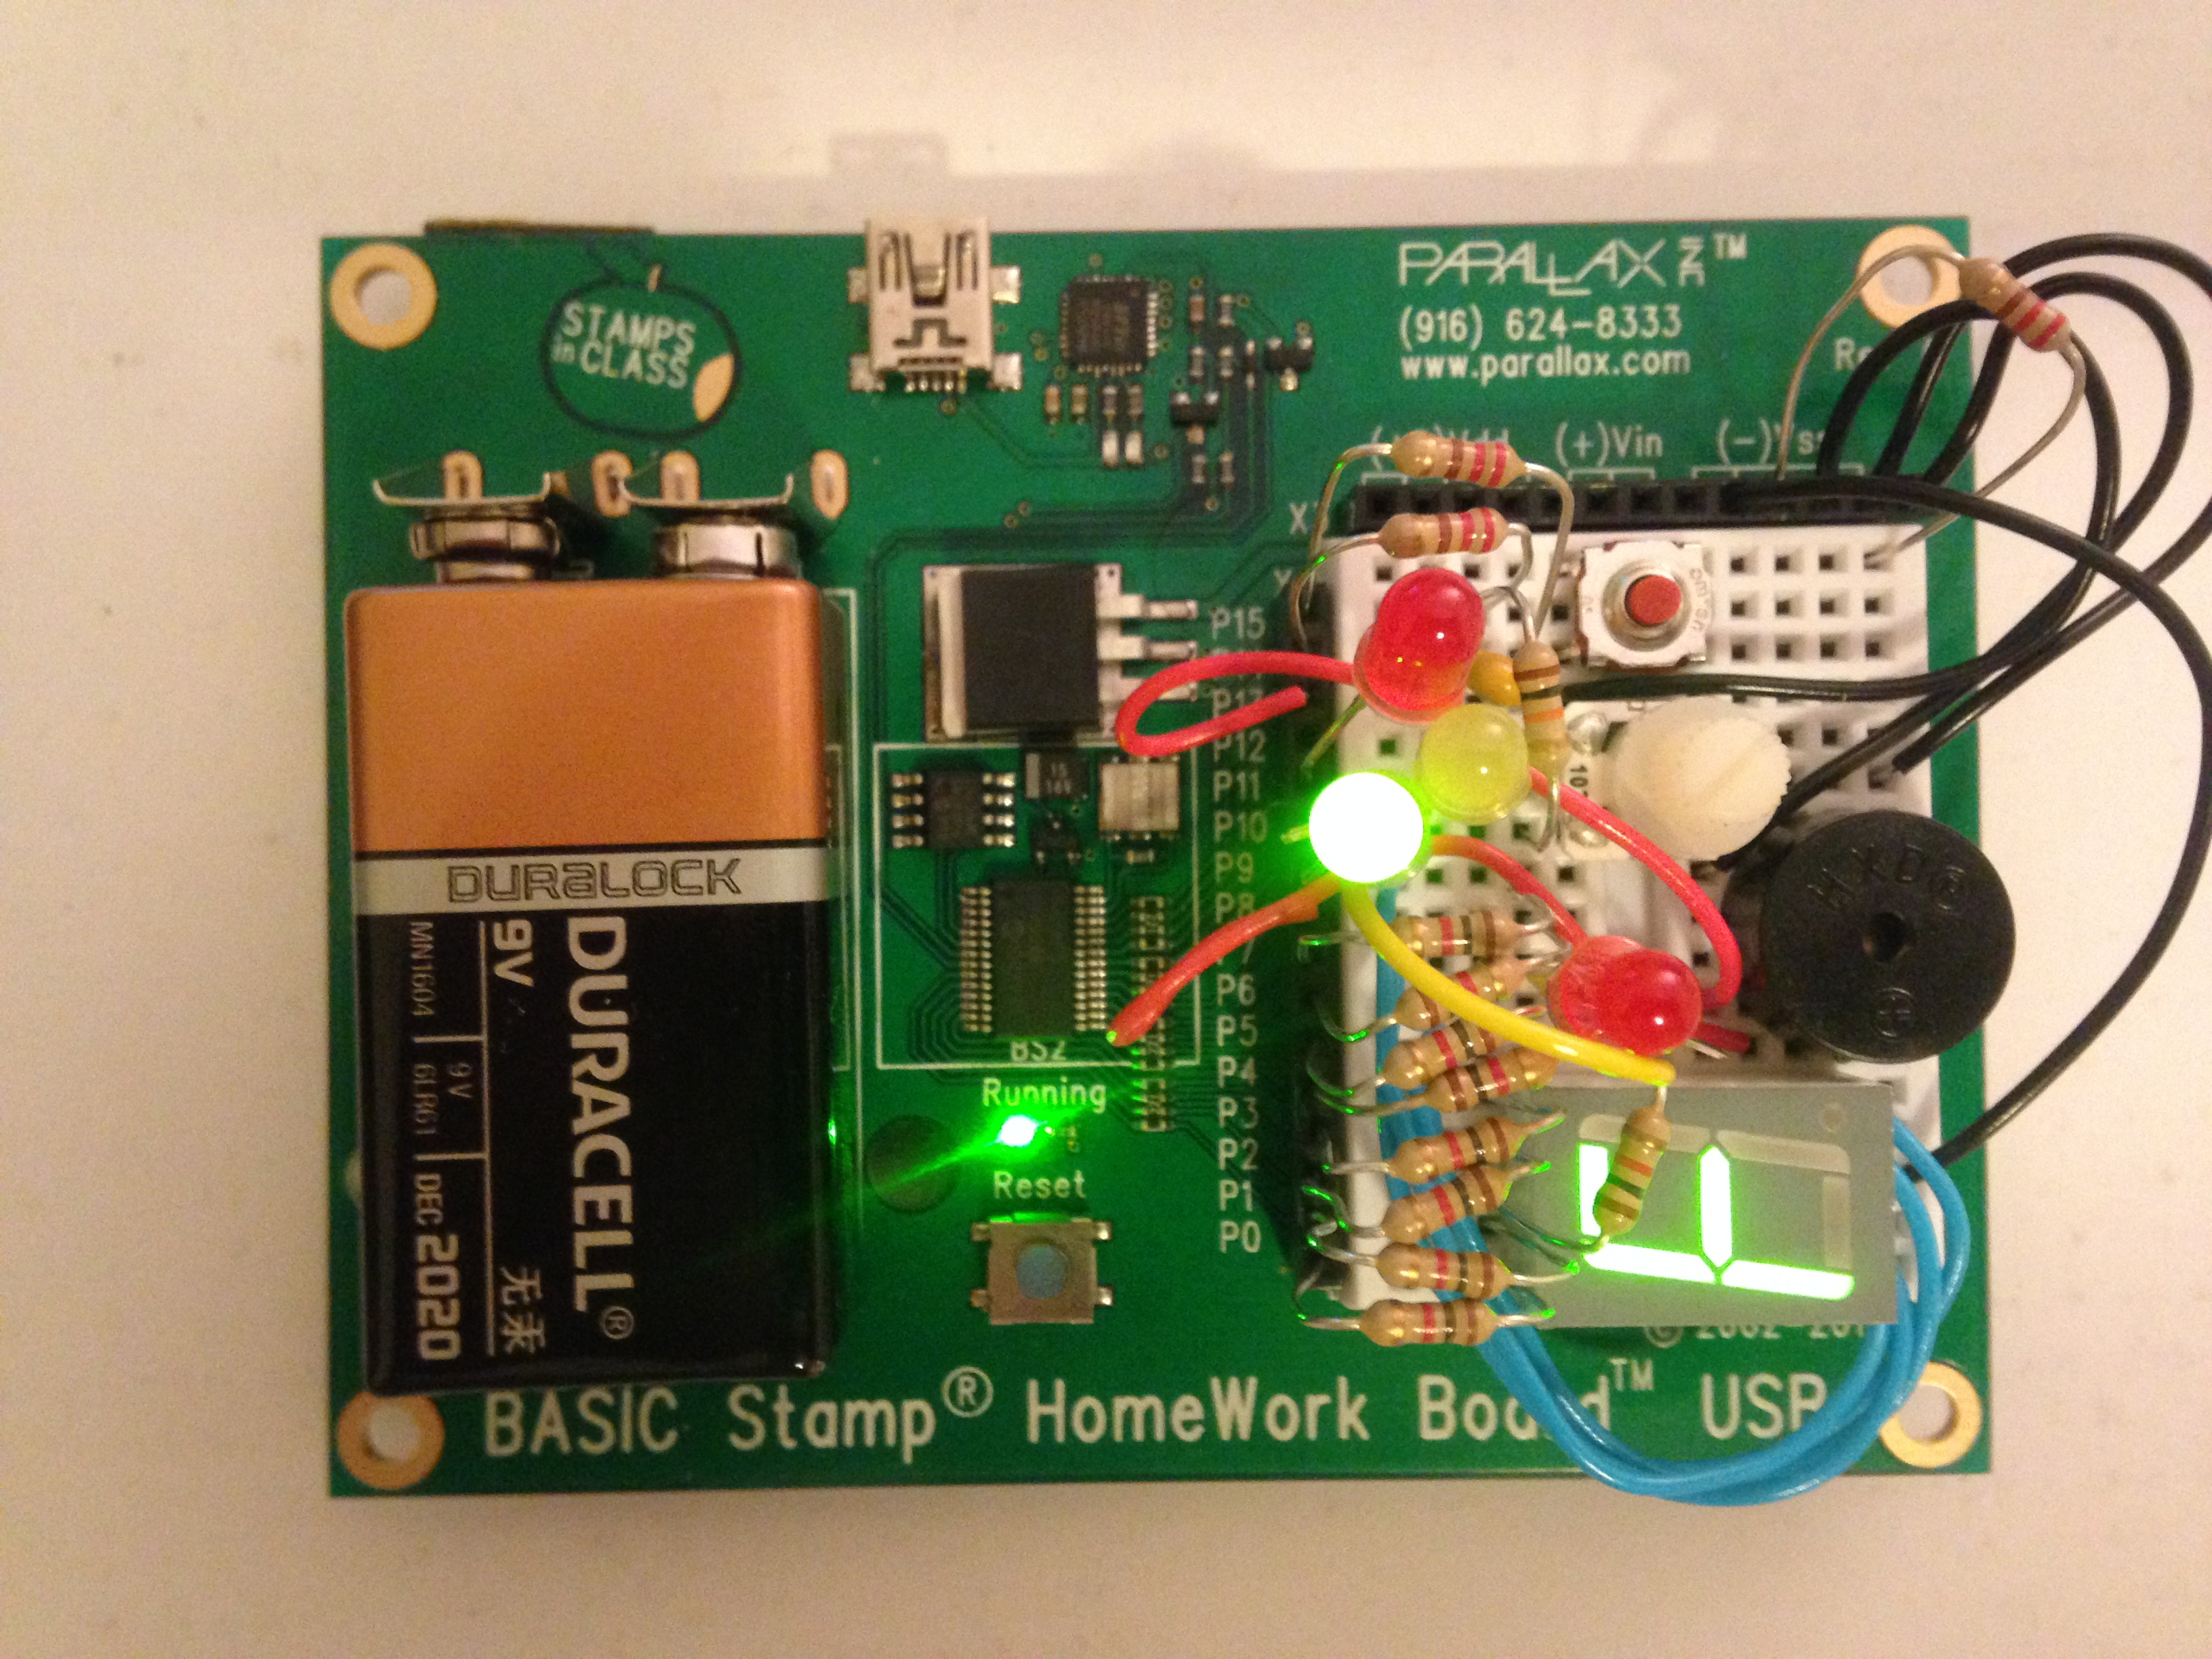
\includegraphics[width=0.6\textwidth]{the-music-trainer.jpg}
\caption{My Music Trainer Playing The Final Countdown}
\label{the-music-trainer}
\end{figure}

\begin{figure}
\centering
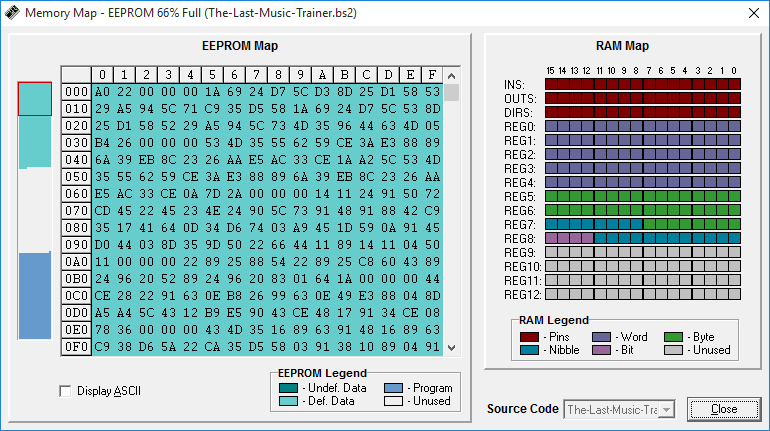
\includegraphics[width=\textwidth]{memory-map.png}
\caption{EEPROM Memory Mapping with Six Songs}
\label{memory-map}
\end{figure}

\section{Discussion}

\subsection{Discussion}

Microcontrollers can easily be used to generate simple tones with
pulse width modulation on digital I/O pins.
Simple songs such as the original cell phone ring tones can be played
as long as more than a single tone at any moment is not required.
(Actually you could play more tones at once with additional pins
and a lower level language).

\section{Exercises}

There were no exercises for this lab.

\clearpage

\section{Implementation Code}

\subsection{The-Last-Music-Trainer.bs2}

\begingroup
\fontsize{10pt}{12pt}
\verbatiminput{The-Last-Music-Trainer.bs2}
\endgroup

\clearpage
\subsection{generate-rtttl-song-data.c}
\label{generate-rtttl-songs-section}

\lstinputlisting[breaklines]{generate-rtttl-song-data.c}



\end{document}
